In this chapter we present some of the numerical results which we have obtained by using the convergent schemes discussed in the previous chapter. We give the results of the following,
\begin{itemize}
	\item
	1D Eikonal Equation
	\item
	Eikonal Equation in 2D.
	\item
	Solving Eikonal Equation on non-rectangular domains using the Immersed Boundary method.
	\item
	Results of the orthographic projection model.
	\item
	Results of the perspective projection model by Prados.	
\end{itemize}

\section{1D Eikonal Equation}
In this section, we present the solution to the most basic Hamilton Jacobi Equation. We use the Godunov Scheme defined in the previous chapter. This scheme converges to the unique viscosity solution, as it is consistent, stable, monotone and the original problem accepts a comparison principle \cite{yong}. Figure (\ref{fig:6}) shows the unique viscosity solution $u(x) = 1-\lvert x \rvert$ to the following Dirichlet Problem.
\begin{eqnarray}
	\lvert u' \rvert &=& 1 \qquad \text{in} \;\; (-1,1)\label{eq:30}\\
	u &=& 0 \qquad \text{on} \;\; \{-1,1\}\label{eq:31}
\end{eqnarray}
\begin{figure}
	\centering
	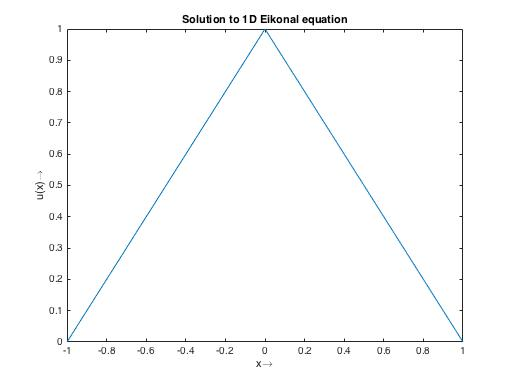
\includegraphics[scale=0.5]{Images/1deik/21.jpg}
	\caption{Viscosity Soution of the 1D Eikonal Equation}
	\label{fig:6}
\end{figure}

\noindent
The next figure (Figure (\ref{fig:7})) shows evolution of the solution to (\ref{eq:30}) - (\ref{eq:31}).\\
\begin{figure}[h!]
	\begin{subfigure}{0.5\textwidth}
		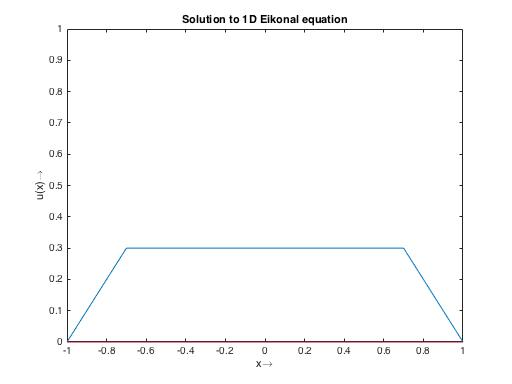
\includegraphics[scale = 0.4]{Images/1deik/3.jpg}
		\subcaption{n = 3 Iterations}
	\end{subfigure}
	\begin{subfigure}{0.5\textwidth}
			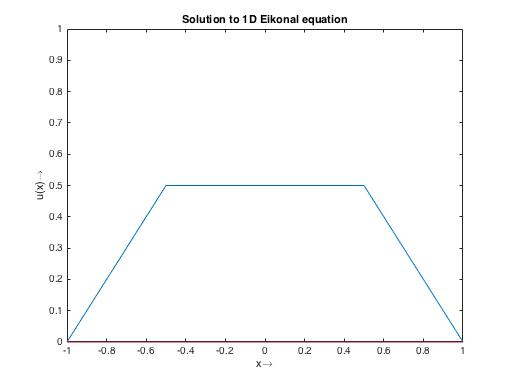
\includegraphics[scale = 0.4]{Images/1deik/5.jpg}
			\subcaption{n = 5 Iterations}
	\end{subfigure}
	\begin{subfigure}{0.5\textwidth}
			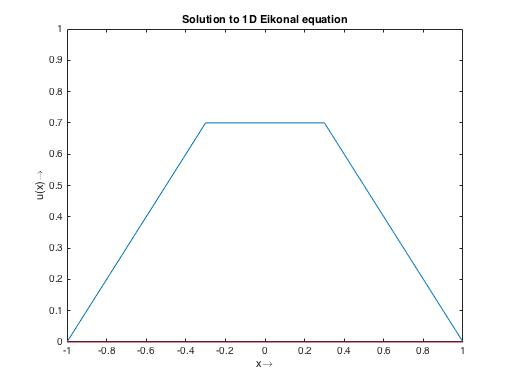
\includegraphics[scale = 0.4]{Images/1deik/7.jpg}
			\subcaption{n = 7 Iterations}
	\end{subfigure}
	\begin{subfigure}{0.5\textwidth}
			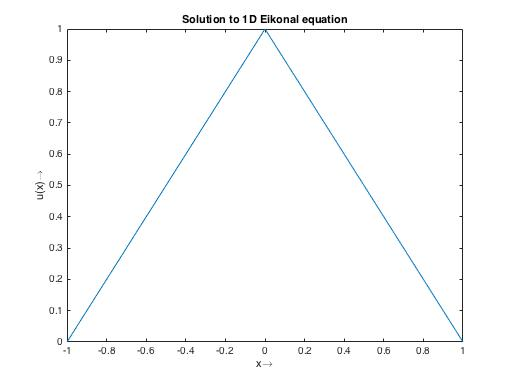
\includegraphics[scale = 0.4]{Images/1deik/21.jpg}
			\subcaption{n = 21 Iterations (Steady State $\epsilon = 10^{-16}$)}
	\end{subfigure}
	\caption{Evolution of solution to the Eikonal Equation. The steady state condition is taken as $\lVert U^{n+1} - u^{n} \rVert < \epsilon = 10^{-16}$}
	\label{fig:7}
\end{figure}

\pagebreak
\section{2D Eikonal Equation}
Next, we show the solution to the Eikonal Equation in 2D for a rectangular domain. For this, we have used the Godunov scheme as well, the fluxes approximating the derivatives along each directions.
\begin{eqnarray}
	\lvert \nabla u \rvert &=& 1 \qquad \text{in} \;\; \Omega = (-1,1) \times (-1,1)\\
	u &=& 0 \qquad \text{on}\;\;\partial \Omega
\end{eqnarray}

\noindent
Figure (\ref{fig:8}) shows the solution to the above Dirichlet Boundary Value Problem. We have taken a $50 \times 50$ mesh to solve the above problem.
\begin{figure}[h!]
	\centering
	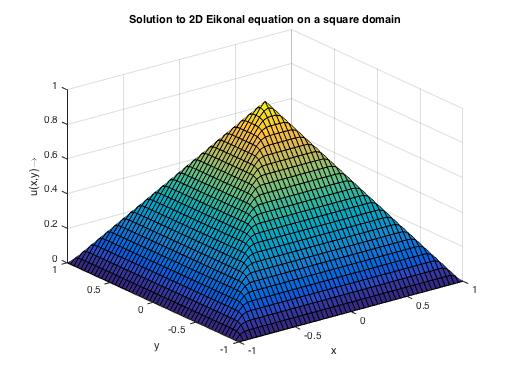
\includegraphics[scale = 0.5]{Images/2D_eik_square.jpg}
	\caption{Solution of 2D Eikonal Equation}
	\label{fig:8}
\end{figure}

\section{Immersed Boundary Method for 2D Eikonal Equations}
So far, the fintie difference techniques can be easily applied to a rectangular cartesian grid. The objective is to extend the same finite difference techniques to a variety other domains, for example - \textit{Circle, L-Domain, Circle with hole} etc. \\

\noindent
To illustrate the technique, we consider a circular domain. For comfort, let us consider a unit circle. We take a rectangular cartesian grid shown in Figure \ref{fig:1} and \textbf{``immerse"} the circluar domain into the rectangular mesh as shown in Figure \ref{fig:2}. This technique is known as the immersed boundary method \cite{pesk} which is widely used to solve problems in Fluid Mechanics.\\

\begin{figure}[h!]
	\centering
	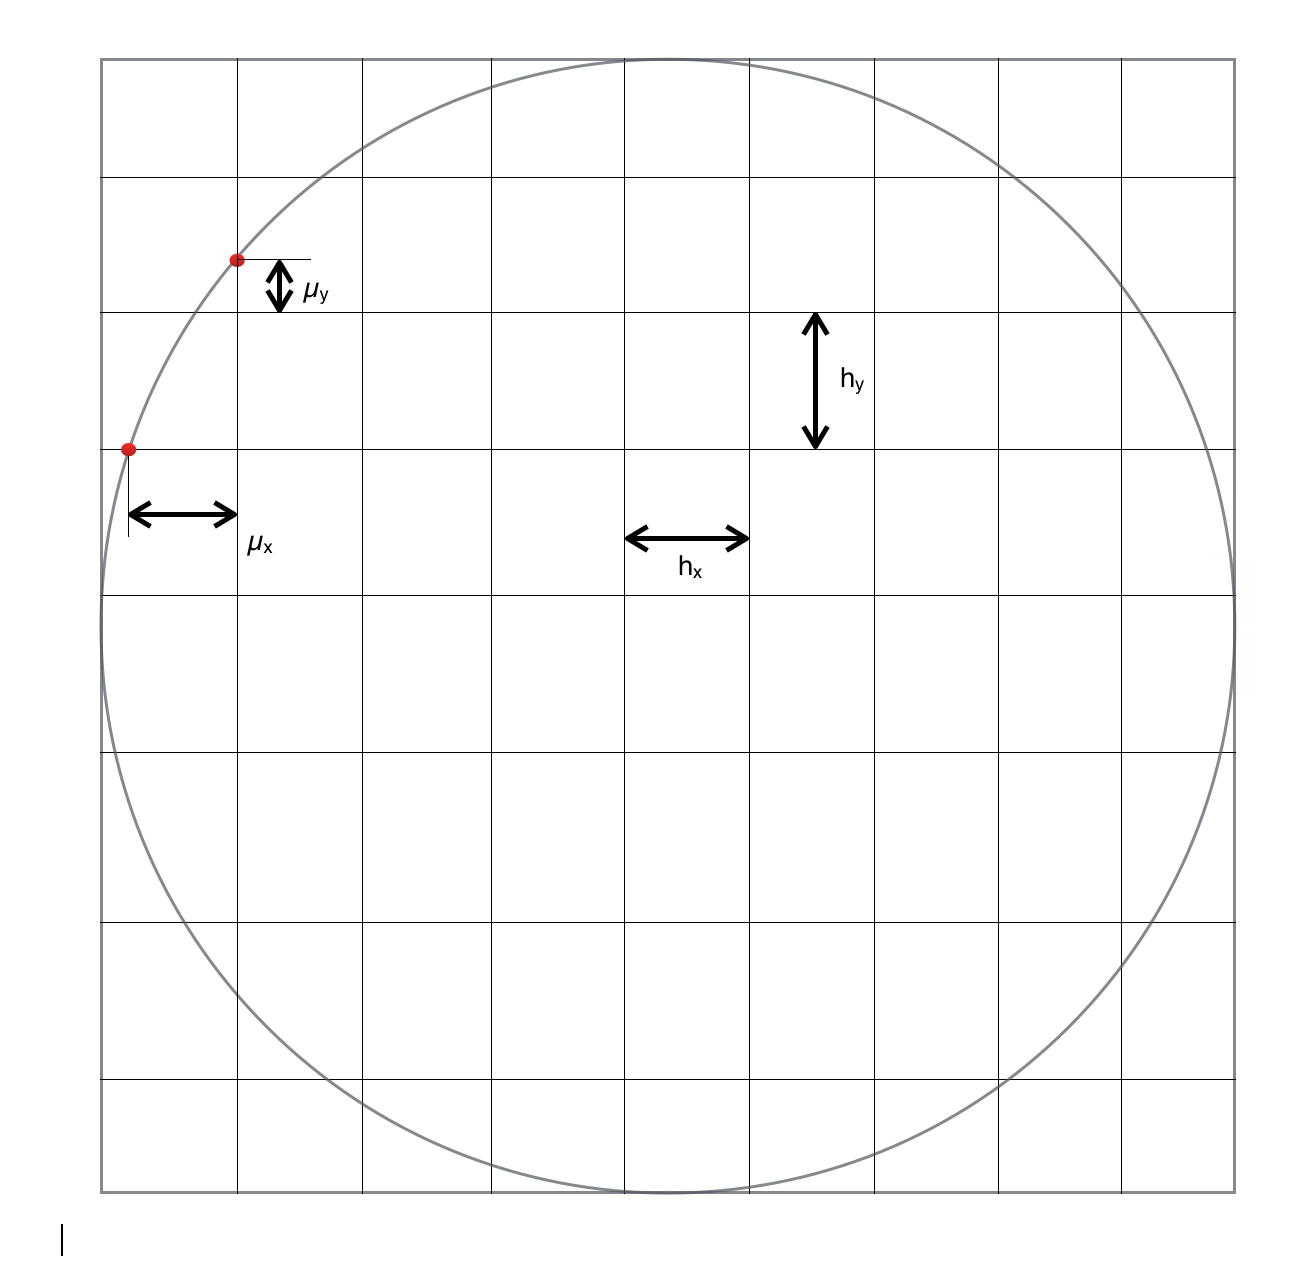
\includegraphics[scale=0.5]{Images/circle-immerse.png}
	\caption{Immersed Circle}
	\label{fig:9}
	\end{figure}
	
	\noindent
	The first challenge in this method is to track the interior and boundary of the 
	immersed domain. For this we introduce a data structure called the \textbf{inout} matrix. The \textbf{inout} matrix is defined as follows,
	\begin{equation}
	inout_{ij} = 
	\begin{Bmatrix}
	0, &\;\; \text{if} \;\; (x_i,y_j) \;\; \text{lies inside the immersed domain}\\
	1, &\;\; \text{otherwise}
	\end{Bmatrix}
	\end{equation}.
	
	\noindent
	The way to track the boundary of the immersed domain using the \textbf{inout} matrix is natural. We simply ignore the grid points whose \textbf{inout} entry is $1$ and set the value $u(x,y) = 0$ at those places. We then solve the eikonal equation using only inside the immersed boundary where the \textbf{inout} value is $0$.\\
	
	\noindent
	To apply the boundary conditions, we are in a position to obtain the points marked in \textbf{red} in Figure \ref{fig:9}. These points are easily obtained by solving the grid lines $x = -1 + ih_x$ or $y = -1 + jh_y$ with the equation of the circle. Note that, from the Dirichlet boundary condition, the value of $u(x,y)$ is prescribed in the problem at these points. \\
	
	\noindent
	When we apply the finite difference formula on the point which is immediately next to the \textbf{red} point - inside the domain, we are in a position to use the distances $\mu_x$ and $\mu_y$ to calculate the finite differences. This is the place where we choose to ignore the points outside the immersed boundary, and take the points that lie on the circle instead.\\
	
	\noindent
	With the distances $\mu_x$ and $\mu_y$, the update formula near the immersed boundary becomes,
	\begin{eqnarray}
	v_{ij}^{n+1} &=& v_{ij}^n - \Delta t\left(\sqrt{D_x^2 + D_y^2}-1\right)\\ 
	D_x &=& max\left(\frac{v_{i+1,j}-v_{i,j}}{\mu_1},\frac{v_{i-1,j}-v_{i,j}}{\mu_2},0\right)\\
	D_y &=& max\left(\frac{v_{i,j+1}-v_{i,j}}{\mu_3},\frac{v_{i,j-1}-v_{i,j}}{\mu_4},0\right)
	\end{eqnarray}
	where $\mu_{1,\dots,4}$ is chosen accordingly, depending on the position of top, bottom, left or right neighboring grid points. If the grid point above the current point, lies on the boundary, then $\mu_3 = \mu_y$ and $\mu_1 =  \mu_2 = h_x, \;\; \mu_4 = h_y$ and so on. There may be cases where two of the neighboring grid points may lie on the boundary. All those cases must be taken proper care of. Results of some numerical experiments are shown in the next chapter.
	
	\subsection{Results}
	Some Numerical Experiments were carried out using the Godunov scheme for a variety of domains.\\
			
		\noindent
		Numerical Experiments were conducted using \textbf{Fortran90} to find out the order of convergence of the scheme with $\epsilon = 10^{-16} \approx$ Machine Error. The \textbf{inout} matrix for a circle with a $10 \times 10$ mesh is shown in Figure \ref{fig:11}
		\begin{figure}[h!]
			\centering
			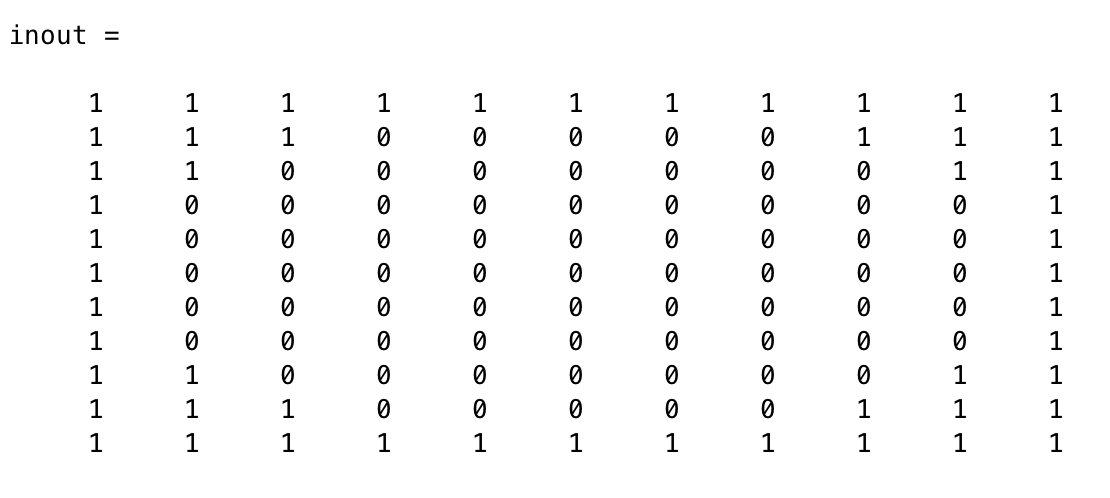
\includegraphics[scale=0.5]{Images/inout.png}
			\caption{\textbf{Inout} Matrix for $10 \times 10$ mesh}
			\label{fig:11}
			\end{figure}\\
			\noindent
			With this \textbf{inout} matrix, we compute the necessary distances near the boundary, for use in the Finite Difference Formula. Following is the profile, obtained when the Godunov Scheme is run for $50 \times 50$ mesh on the master rectangle with steady state $\epsilon = 10^{-16}$.
			\begin{figure}[h!]
				\centering
				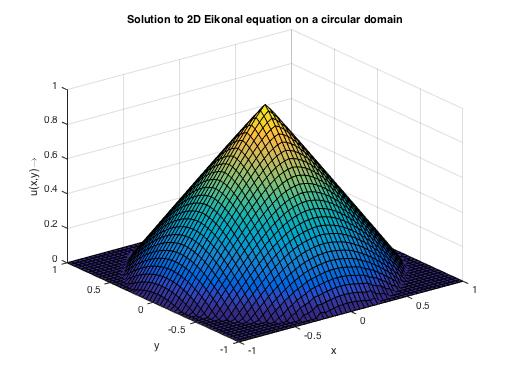
\includegraphics[scale = 0.5]{Images/2D_eik_circle.jpg}
				\caption{Solution in a circular domain}
				\label{fig:5}
				\end{figure}\\
				
				\noindent
				Using \textbf{Fortran90}, order of convergence analysis was performed on the scheme and the results are tabulated.\\
				\begin{center}
					\begin{tabular}{|c|c|c|}
						\hline
						N & Error & Order of Convergence\\
						\hline
						10 & 0.9878E-01 & 0.685 \\
						\hline
						20 & 0.6145E-01 & 0.728 \\
						\hline	
						40 & 0.3710E-01 & 0.738 \\
						\hline	
						80 & 0.2223E-01 & 0.761 \\
						\hline	
						160 & 0.1311E-01 & 0.783 \\
						\hline	
						320 & 0.0762E-01 & 0.800  \\
						\hline
						640 & 0.0437E-01 & -\\
						\hline
						\end{tabular}
						\end{center}
						
						\noindent
						The same method can be used to generate profiles for a variety of domains as shown. The idea is to tweak the \textbf{inout} matrix corresponding to the shape of the domain and appropriately take care of the immersed boundary grid points.\\
						
						\begin{figure}[h!]
							\begin{subfigure}{.5\textwidth}
								\centering
								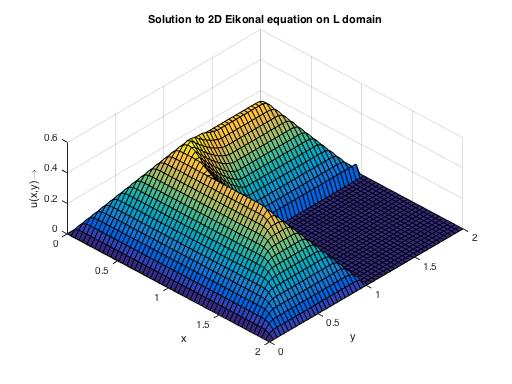
\includegraphics[scale = 0.45]{Images/2D_eik_Ldomain.jpg}
								\caption{L-Domain}
								\label{fig:12}
								\end{subfigure}
								\begin{subfigure}{.5\textwidth}
									\centering
									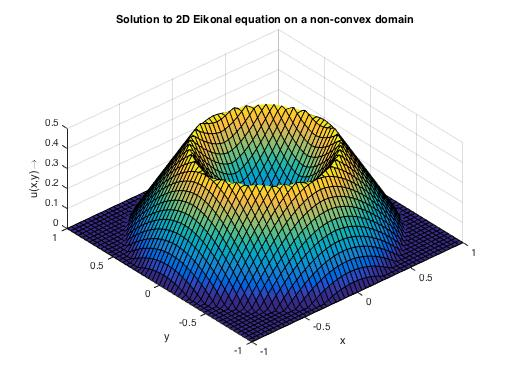
\includegraphics[scale = 0.45]{Images/2D_eik_hole.jpg}
									\caption{Circle with a hole in the middle}
									\label{fig:13}
									\end{subfigure}
									\caption{Other Domains}
									\end{figure}
									
									\noindent
									Figure \ref{fig:12} and Figure \ref{fig:13} shows the profile that is obtained when the Immersed Boundary Technique is applied to solve the Eikonal Equation on a L-Shaped Domain and a circle with a hole in it (non-convex domains) respectively. Similar Experiments can be conducted to model various problems in a variety of domains.

\section{Orthographic Projection}
For the orthographic projection model \cite{rouy}, the Eikonal Type HJE, is given by 
\begin{eqnarray}
	\lvert \nabla u \rvert = \sqrt{\frac{1}{I(x)^2} - 1}\label{eq:ortho}
\end{eqnarray}
where $I(x)$ is the intensity function of the input image. Following test was carried out to verify the model using a synthetic image of a vase shown in Figure (\ref{fig:14}). 
\begin{figure}[h!]
	\centering
	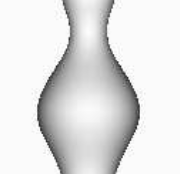
\includegraphics[scale = 1.5]{Images/vase.png}
	\caption{Synthetic Test Vase}
	\label{fig:14}
\end{figure}

\noindent
(\ref{eq:ortho}) was solved with a Homogeneous Neumann Boundary Condition on $\partial \Omega$ and the result is presented below. The equation was solved using the Godunov upwind scheme.
\begin{figure}[h!]
	\centering
	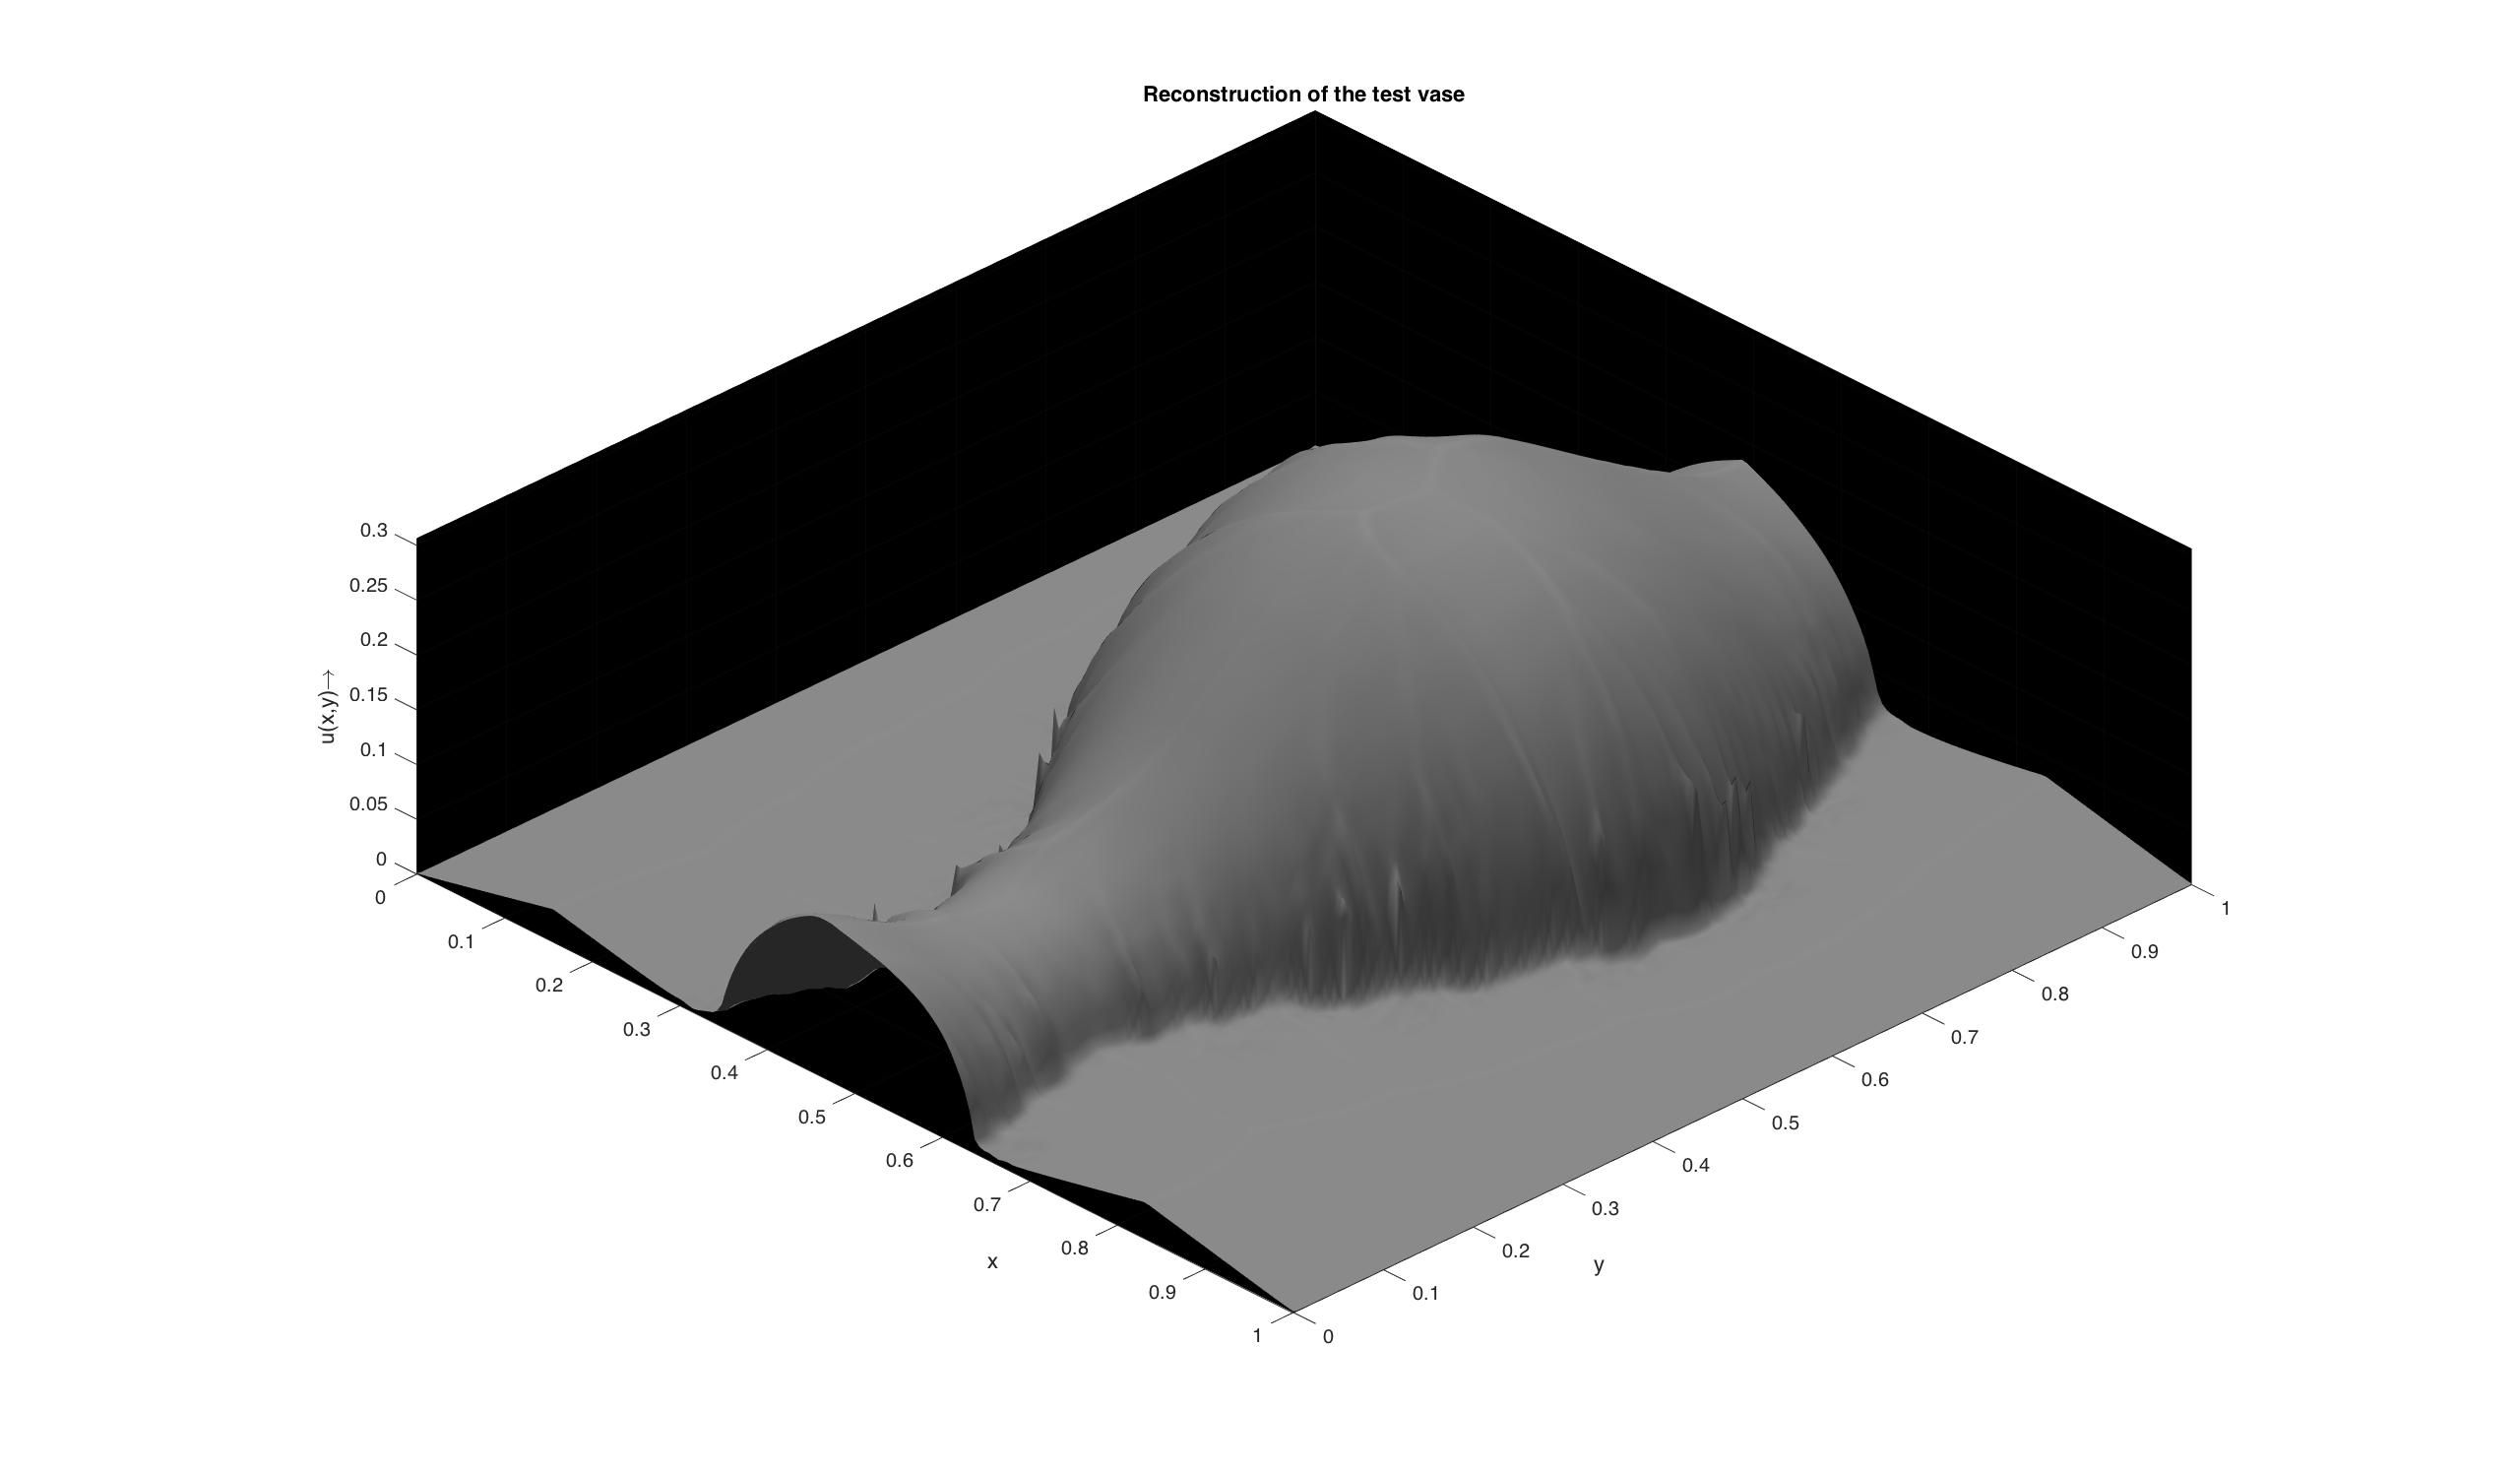
\includegraphics[scale = 0.15]{Images/vase.jpg}
	\caption{Reconstruction of the Synthetic Test Vase}
	\label{fig:15}
\end{figure}

\section{Perspective Projection Model}
The HJE\cite{prados2} governing the Perspective Projection Model is given by
\begin{eqnarray}
	-e^{-2v} + \frac{I(x)f^2}{Q(x)} \sqrt{f^2|\nabla v|^2 + (x.\nabla
		v)^2 + Q(x)^2} = 0 \qquad \text{in} \;\;\; \Omega
\end{eqnarray}

\noindent
We solve this equation by adding a transient $v_t$ term and then solve till we reach the steady state.
\begin{eqnarray}
v_t -e^{-2v} + \frac{I(x)f^2}{Q(x)} \sqrt{f^2|\nabla v|^2 + (x.\nabla
	v)^2 + Q(x)^2} = 0 \qquad \text{in} \;\;\; \Omega
\end{eqnarray} 

\noindent
To solve the time-dependent problem, we take the constant initial condition
\begin{equation}
	v_0 = -\frac{1}{2}\ln(\min_{x\in\Omega} I(x)f^2)
\end{equation}
to ensure convergence to the solution as discussed in Chapter 4. Refer \cite{prados2} for more details. We used the intensity image and attempted to reconstruct the original 3D shape. The input image along with the reconstructed images are shown in Figure (\ref{moz}). Steady State was taken to be $\lVert U^{n+1} - U^n \rVert < 10^{-16}$.
\begin{center}
	\begin{figure}
	\begin{subfigure}{0.5\textwidth}
		\centering
		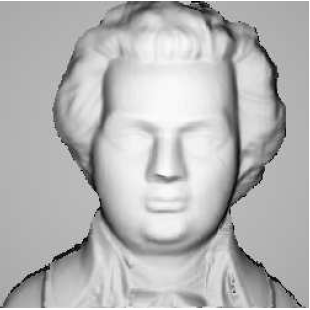
\includegraphics[scale = 0.85]{Images/moz.png}
		\caption{Intensity Image for Mozart}
	\end{subfigure}
	\begin{subfigure}{0.5\textwidth}
				\centering
				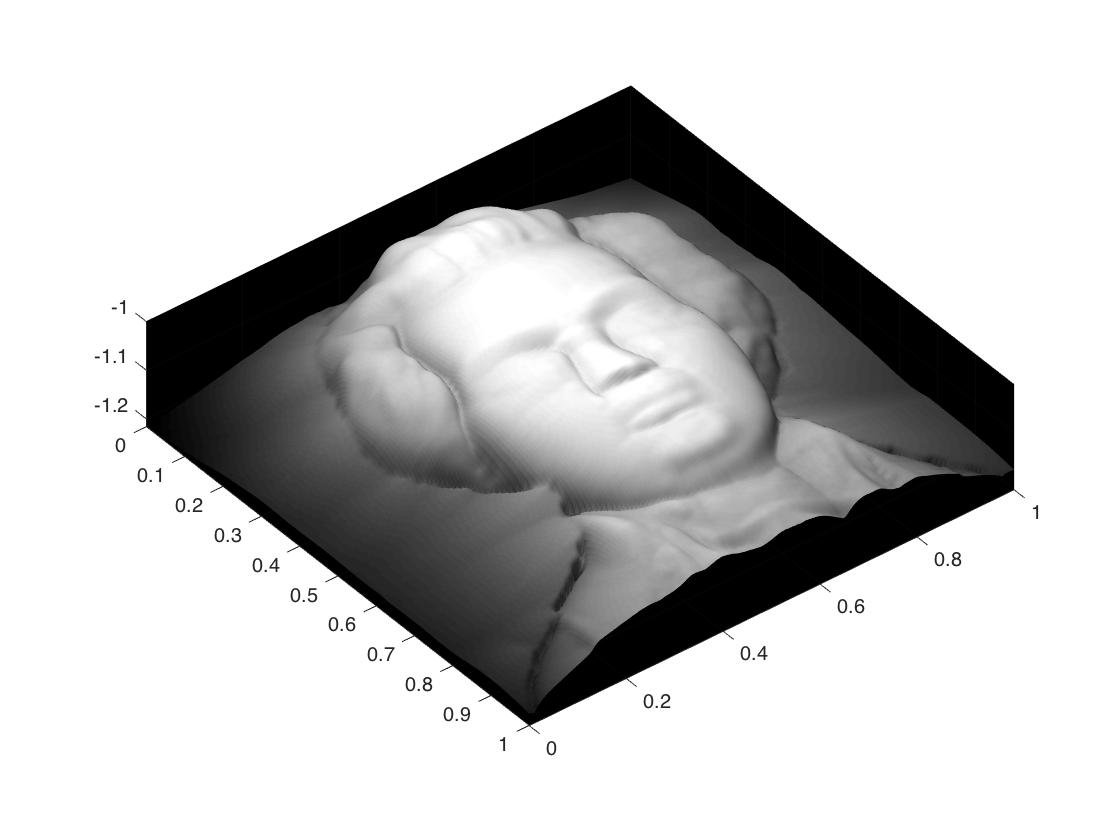
\includegraphics[scale = 0.24]{Images/moz.jpg}
				\caption{Reconstructed Face of Mozart}
	\end{subfigure}
		\begin{subfigure}{0.5\textwidth}
			\centering
			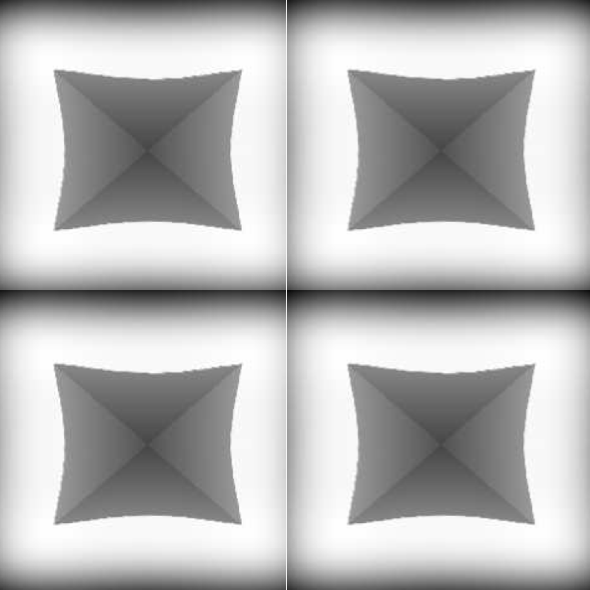
\includegraphics[scale = 0.5]{Images/thing4.png}
			\caption{Intensity Image for Test}
		\end{subfigure}
		\begin{subfigure}{0.5\textwidth}
			\centering
			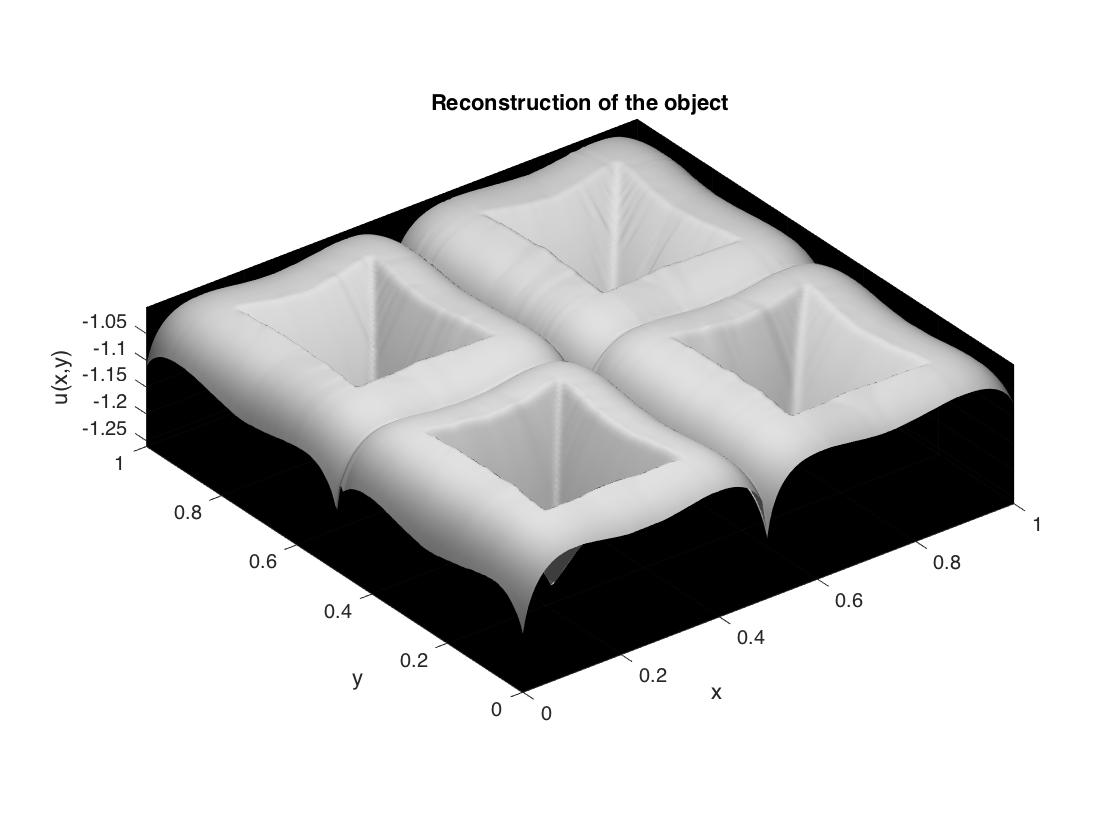
\includegraphics[scale = 0.24]{Images/thing4.jpg}
			\caption{Reconstructed Test Image}
		\end{subfigure}
	\caption{Reconstruction using Perspective Model by Prados \cite{prados2}}
	\label{moz}
\end{figure}
\end{center}
\noindent
The time evolution of the Mozart Face is shown in Figure (\ref{fig:evol}). 
\begin{center}
	\begin{figure}
		\begin{subfigure}{0.5\textwidth}
			\centering
			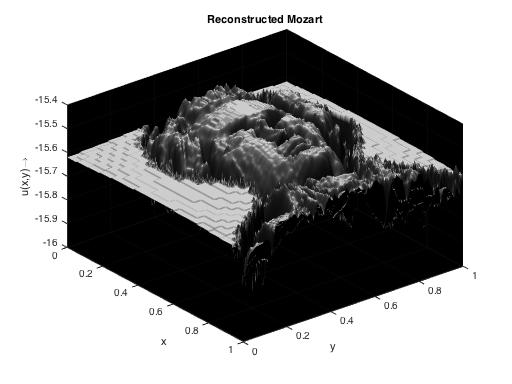
\includegraphics[scale = 0.4]{Images/moz/moz_100.jpg}
			\caption{100 Iterations}
		\end{subfigure}
		\begin{subfigure}{0.5\textwidth}
			\centering
			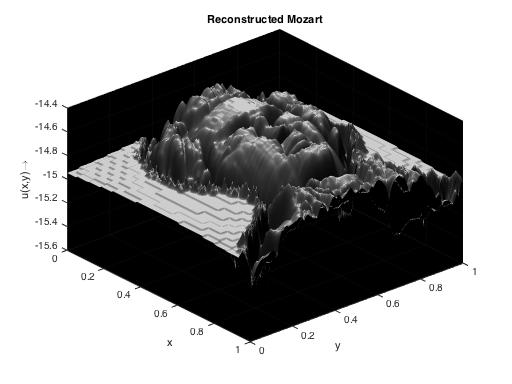
\includegraphics[scale = 0.4]{Images/moz/moz_300.jpg}
			\caption{300 Iterations}
		\end{subfigure}
		\begin{subfigure}{0.5\textwidth}
			\centering
			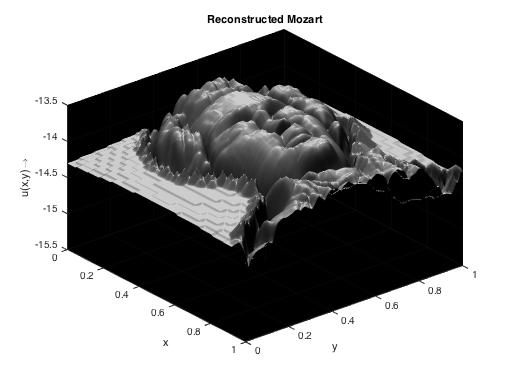
\includegraphics[scale = 0.4]{Images/moz/moz_500.jpg}
			\caption{500 Iterations}
		\end{subfigure}
		\begin{subfigure}{0.5\textwidth}
			\centering
			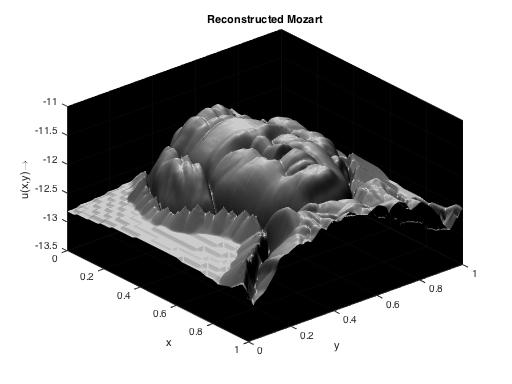
\includegraphics[scale = 0.4]{Images/moz/moz_1000.jpg}
			\caption{1000 Iterations}
		\end{subfigure}
		\begin{subfigure}{0.5\textwidth}
			\centering
			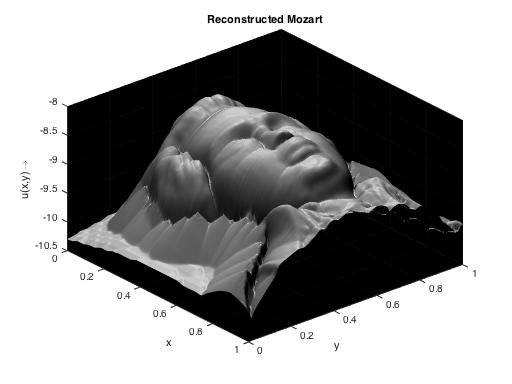
\includegraphics[scale = 0.4]{Images/moz/moz_2000.jpg}
			\caption{2000 Iterations}
		\end{subfigure}
		\begin{subfigure}{0.5\textwidth}
			\centering
			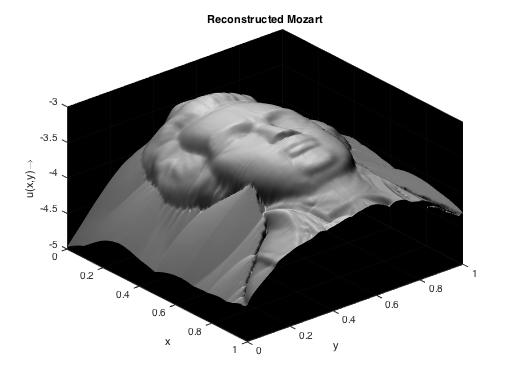
\includegraphics[scale = 0.4]{Images/moz/moz_5000.jpg}
			\caption{5000 Iterations}
		\end{subfigure}
		\caption{Time evolution of Mozart's Face}
		\label{fig:evol}
	\end{figure}
\end{center}

\noindent
\begin{center}
	\begin{figure}
		\begin{subfigure}{0.5\textwidth}
			\centering
			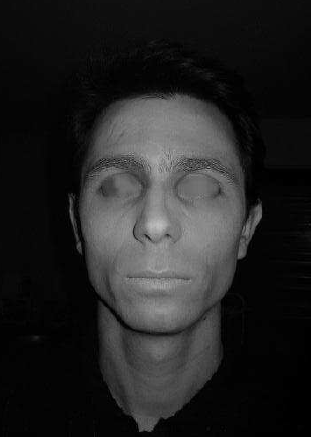
\includegraphics[scale = 0.35]{Images/realface/gleb_closed.png}
			\caption{Input Image for Real Face}
		\end{subfigure}
		\begin{subfigure}{0.5\textwidth}
			\centering
			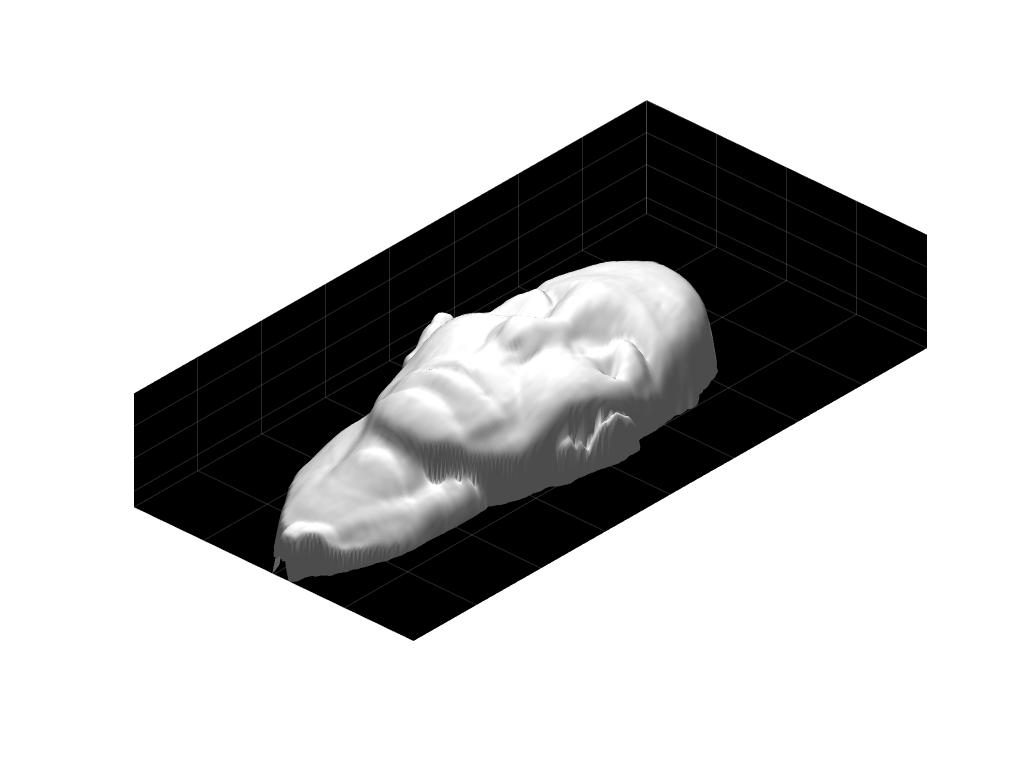
\includegraphics[scale = 0.2]{Images/realface/gleb_closed.jpg}
			\caption{Reconstructed}
		\end{subfigure}
		\begin{subfigure}{0.5\textwidth}
			\centering
			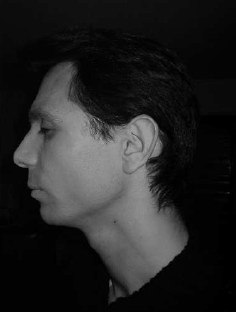
\includegraphics[scale = 0.902]{Images/realface/gleb_side.png}
			\caption{Input image for side view}
		\end{subfigure}
		\begin{subfigure}{0.5\textwidth}
			\centering
			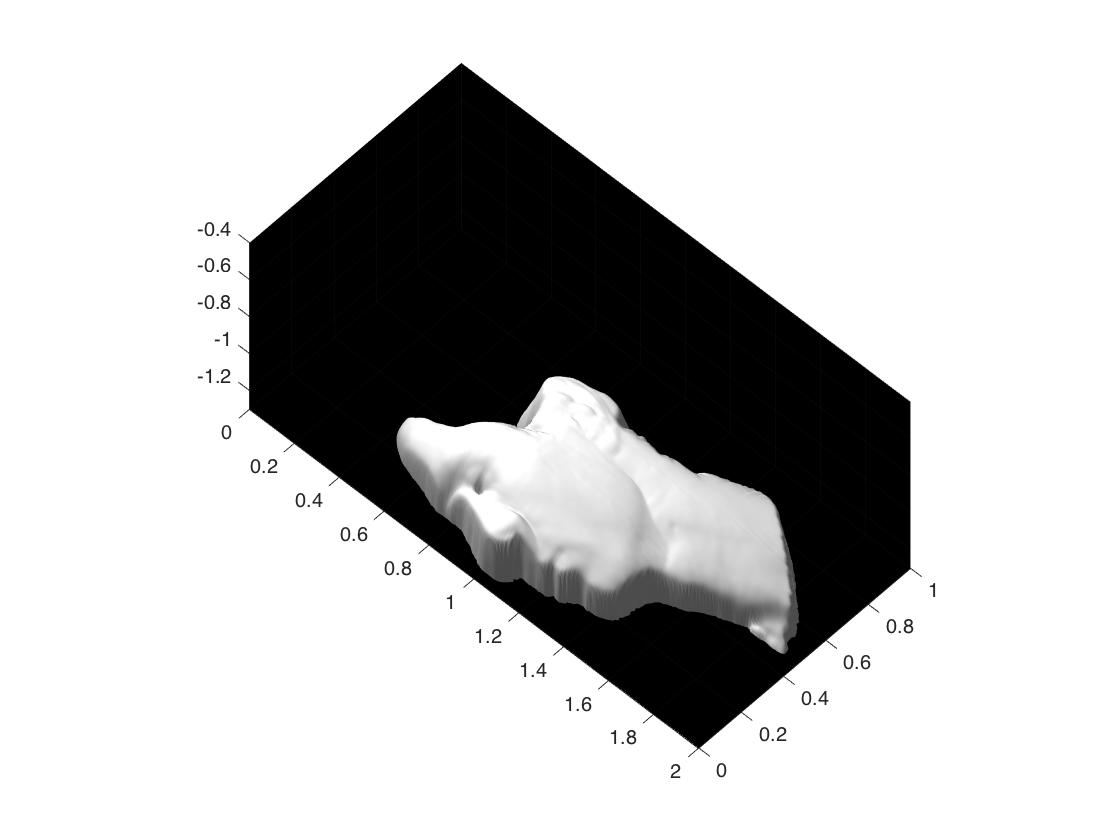
\includegraphics[scale = 0.2]{Images/realface/gleb_side.jpg}
			\caption{Reconstructed}
		\end{subfigure}
		\begin{subfigure}{0.5\textwidth}
			\centering
			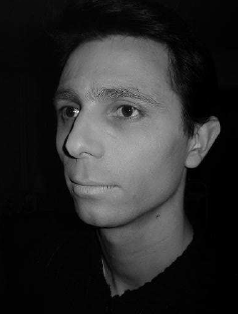
\includegraphics[scale = 0.902]{Images/realface/gleb_oblique.png}
			\caption{Input image for oblique view}
		\end{subfigure}
		\begin{subfigure}{0.5\textwidth}
			\centering
			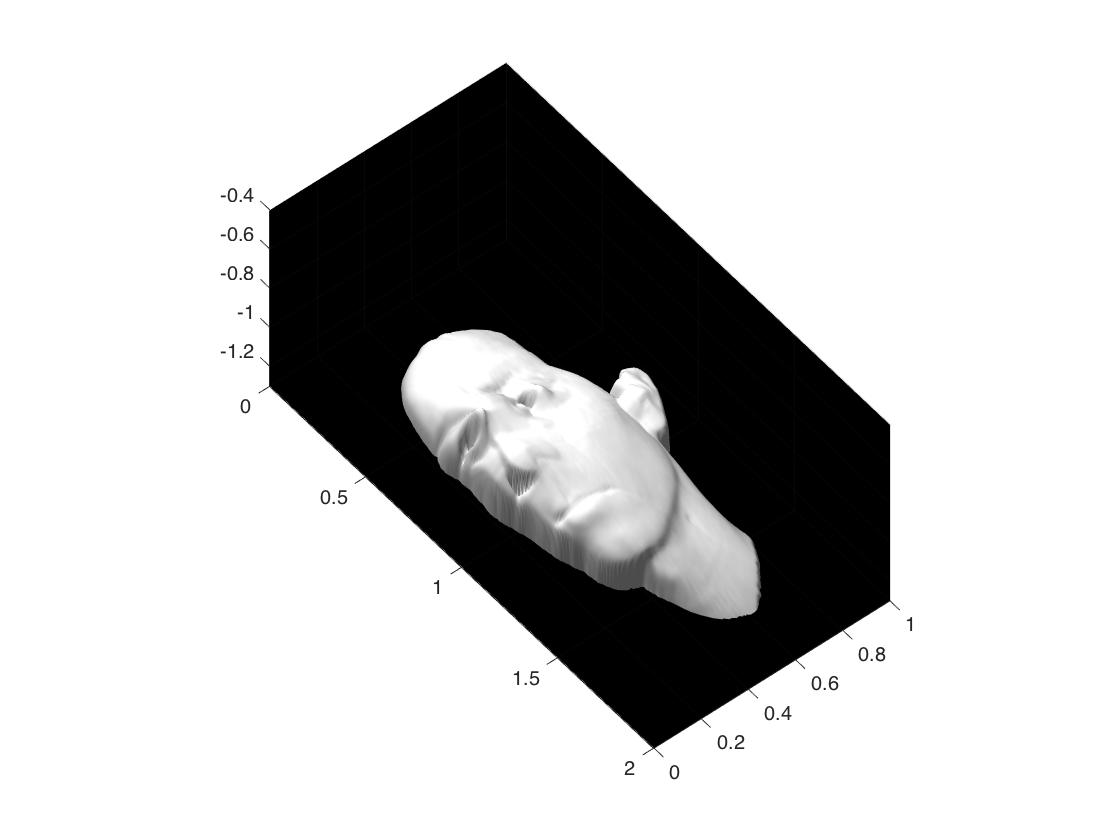
\includegraphics[scale = 0.2]{Images/realface/gleb_oblique.jpg}
			\caption{Reconstructed}
		\end{subfigure}
		\caption{Real Life Reconstructions}
		\label{fig:real}
	\end{figure}
\end{center}
 